\chapter{General Information}

\label{chap:introduction}

\section{Scope}
SHeavy will only handle contagious and lethal epidemics. It is designed for
worldwide use among governments, health organisations, hospitals and citizens.
This document provides information about what the software is intended to do and how to us it.
Furthermore it includes our web-interface only for professional users and the
mobile interface for both, professional and normal users. This document does not
contain any source code of the program and is not intended to help users reverse
engineer our programs.\\

\section{Purpose}
This document is the user manual of the program SHeavy (v0.5) . It was
realized to introduce our program and its features to its possible users. It
defines which type of users have access to which functions and information of the program.\\

\section{Intended audience}
SHeavy is targeting governments, health organisations, hospitals or in general
any type of users who could help in solving such a epidemic crisis. It can be
technicians with computer science competences or higher level implied people 
like investors, governements or any other person with specific competences in a
specific domain.\\

Furthermore SHeavy is also targeting people who aren't directly concerned with
the management of a epidemic crisis but people who are interested in accessing
information about the crisis. These persons are defined as normal users. In any
moment they are going to interact with the management systems in order to send
instructions or information except of their GPS locations.\\

\section{SHeavy}
SHeavy is a software developed by CrisYs Corp whose goal is to predict and
give advices to handle worldwide and lethal epidemics. It will analyse data
shared by doctors around the world and deduce whether there is a beginning of
epidemic. Predictions about its growth will be made and the relevant actors will
be notified to take adequate measures to restrain that growth and treat it as
soon as possible. The system will also keep logs of all the communications and
the actions carried out.\\

\subsection{Actors \& Functionalities}
SHeavy has different functionalities for several Actors. For this purpose an
hierachical chart is given below.\\

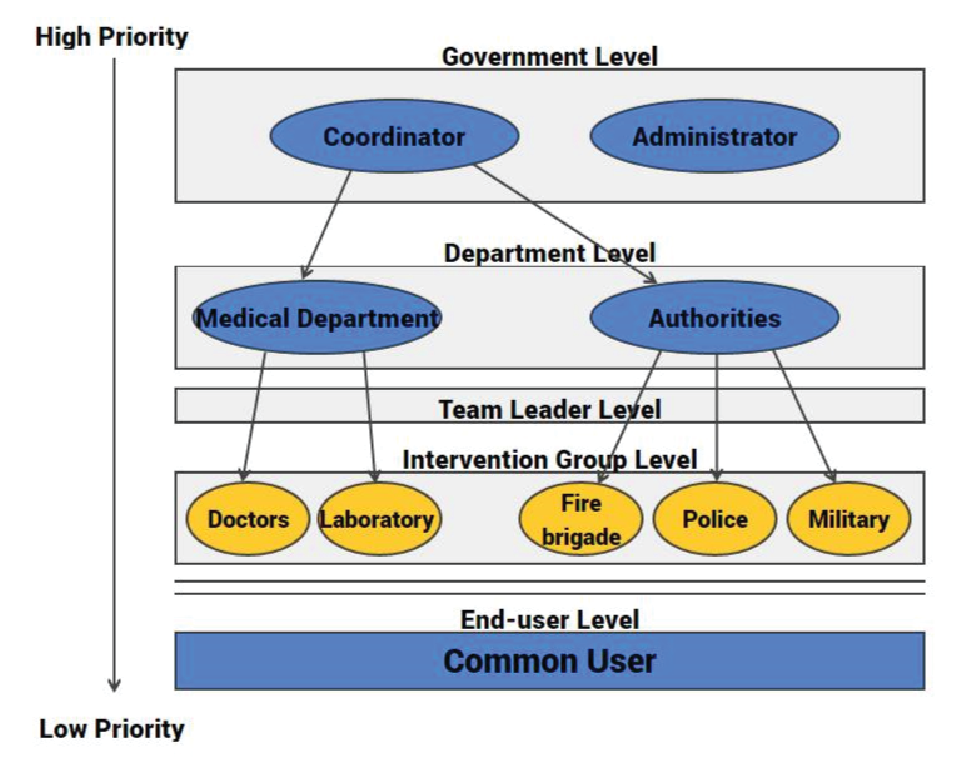
\includegraphics{images/ActorLevels.eps} \\

\subsubsection{CrisYs Corp}
CrisYs Corp are the developers of the crisis management system SHeavy.\\
\begin{description}
 \item[$\bullet$] Create and set up the system.
\end{description} 

\subsubsection{Common Users}
A common user is defined as an end user who uses SHeavy only in order to
collect information about the possible epidemic and uses the given instructions
to avoid the infection.\\
\begin{description}
 \item[$\bullet$] Common users are the principle target of SHeavy. They are
 going to use the application in order to reach information about a possible
 or several epidemic and follow the instructions given by SHeavy. 
 \item[$\bullet$]Common users will get warnings if accessing an infected
zone by GPS tracking. They will have paths to follow to access and find the
safe zones.
\end{description}

\subsubsection{Coordinators}
The Coordinator is the intermediate between its two low-level departements,
Medical Departement and Authorities, and the Government. He will execute the
orders of the Government by using SHeavy. The Coordinator has several main
functions such as :
\begin{description}
 \item[$\bullet$] The Coordinator starts or beends the alert of the concerning
 epidemic.
 \item[$\bullet$] He's also responsable for the Ressources Management, which is
 already set up before the epidemic.
 \item[$\bullet$] Another task is to update SHeavy's Map accordingly to the
 situation.
\end{description} 

\subsubsection{Administrator}
The Administrator is the responsable who keeps the ssystem operational.
Additionly he distributs the logins and the professional web and mobile
interface.
\begin{description}
 \item[$\bullet$] The Administrator keeps the system operational by maintaining
 the system.
 \item[$\bullet$] If necessary he performs some improvements and bugs
 corrections.
 \item[$\bullet$] The Administrator distributs the professional web and mobile
 interface to the concerned persons. and also the logins.
 \item[$\bullet$]  The admistrator is able to block a mobile phone or desktop
 interface for the security of the system.
\end{description} 

\subsubsection{Medical Departement}
The Medical Departement has two main groups, namely Doctors and the Laboratory.
Each one is connected with each other and they are exchanging their reports. The
Medical Departement is the intermediate between its groups and the Coordinator.
\begin{description}
 \item[$\bullet$] Sends an alert of a possible epidemic to the Coordinator.
 \item[$\bullet$] Sends several reports to the Coordinator.
\end{description} 

\subsubsection{Doctors}
Doctors are in charge of taking care of the infected victims. They'll also
perform check ups and send reports and blood sample to the Laboratory.
\begin{description}
 \item[$\bullet$] Write reports that will be sent to the Laboratory and Medical
 Departement.
 \item[$\bullet$] Works in various check points or hospitals in order to perfom
 check ups.
 \item[$\bullet$] Take care of the infected patients the time that an antivirus
 is found.
 \item[$\bullet$] Takes blood sample from the infected patients and sends them
 to the Laboratory.
\end{description} 

\subsubsection{Laboratory}
The Laboratory is a medical group which goal is to find a cure against the
virus. In constant collaboration with different medical chiefs they will get
relevant information of the evolution of the epidemic in realtime. They also get the
blood samples and reports from the Doctors.
\begin{description}
 \item[$\bullet$] Write reports that will be sent to the Doctors and Medical
 Departement.
 \item[$\bullet$] Analizing the blood samples to isolate the virus and demantle
 its structure to provide an antivirus.
 \item[$\bullet$] Gives a guideline to the application as a news so that all the
 people knows how to protect itself from become infected.
\end{description} 

\subsubsection{Authorities}
The Authorities is regrouping various intervention groups such as the fire
brigade, the police and the militaries. They are working together and have a
connection with each other. The Authorities are the intermediate between its
groups and the Coordinator.
\begin{description}
 \item[$\bullet$] Support group for various purposes. 
\end{description}

\subsubsection{Team Leader}
Team Leader are present in all instances of epartements such as Medical
Departements and Authorities. They are the leader of an intervention group which
is going to execute missions given by the Coordinator.
\begin{description}
 \item[$\bullet$] They are responsable of his team.
 \item[$\bullet$] Accept or decline a mission given by the Coordinator.
 \item[$\bullet$] Execute missions.
\end{description}

\subsection{Operating environment}
SHEAVY is a webbased application. It has a server and a client side. The server
needs to be powerfull to handle the mass of information. Clients need to have a
good internet access and a basic system requirement to access fast their
pages.\\

\subsubsection{System requirements: Client}
\begin{tabular}{|c|c|}
\hline
\multicolumn{2}{|c|}{\textbf{Phone Application}} \\
\hline
\multicolumn{2}{|c|}{\textit{\textbf{Android}}} \\
\hline
OS & Android \\
\hline
Hardware & ARM 5 Dual Core \\
\hline
\multicolumn{2}{|c|}{\textit{\textbf{iOS}}} \\
\hline
Operating System & iOS 8 \\
\hline
Hardware & iPhone 5 \\
\hline
\end{tabular}

\subsubsection{System requirements: Server}
\begin{tabular}{|c|c|}
\hline
\multicolumn{2}{|c|}{\textbf{Server Application}} \\
\hline
\multicolumn{2}{|c|}{\textit{\textbf{Linux x86/x64}}} \\
\hline
Kernel & 4.8.1 \\
\hline
Hard disk space & 10 TB   \\
\hline
Processeur & Intel Xeon E7-8893 \\
\hline
RAM & 32 GB \\
\hline
\end{tabular}

\section{Document structure}  
Information on how this document is organised and it is expected to be
used. Recommendations on which members of the audience
should consult which sections of the document, and explanations about the used
notation (i.e. description of formats and conventions) must also be provided.\\

You will find in chapter one all the necessary and general information to be properly introduced
to the system we develop. Chapter two includes more detailed materials covering the main
use-cases we implements, involving actors and basic technical details. Chapter three is set
aside for more advanced readers, with technical skills particular to programming or at least
understanding what it is about.
For special notations and complex words please have a look at the glossary at the end of the
document.\\






